\subsection{Basics of decision trees}

A typical decision tree looks as in image \ref{fig:3_tree_example}.

\begin{figure}[h]
  \centering
  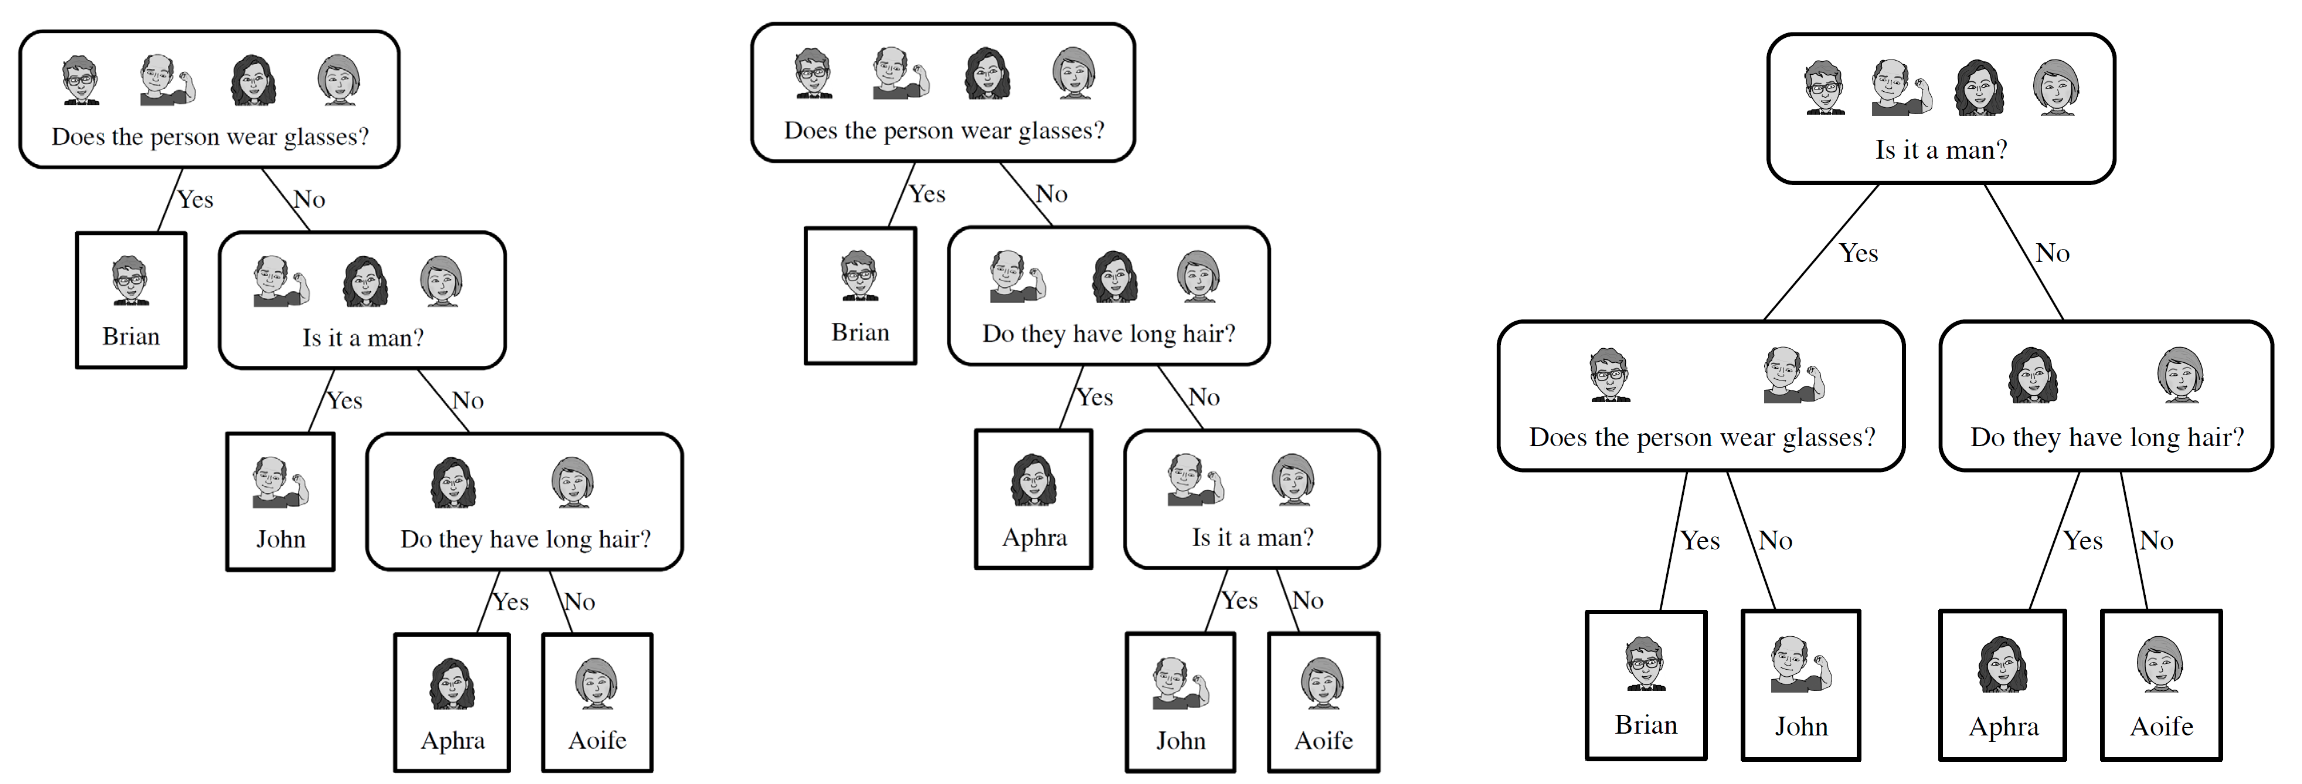
\includegraphics[width=0.9\textwidth]{assets/trees/basics/tree_example_people.png}
  \caption{Decision tree for person distinction (different grouping)}
  \label{fig:3_tree_example}
\end{figure}

The example shows that a \textbf{decision tree}\sidenote{Decision tree} is built by \textbf{grouping} instances step by step. In general, instances are partitioned into \textbf{increasingly smaller groups}. 
\begin{itemize}
  \item How the groups are formed decides the outcome of the concrete decision tree (different trees are possible).
  \item For the grouping, keep two goals in mind:
  \begin{enumerate}
    \item The tree shall be as small and simple as possible.
    \item The leaves shall be homogeneous in terms of the target feature.
  \end{enumerate}
\end{itemize}

The overall \textbf{goal of a decision tree} is to explain the target feature in terms of the descriptive features, so we have a supervised learning scenario.
\begin{itemize}
  \item For categorical features we can differentiate based on the different classes.
  \item For numerical features, we need to define a threshold or something similar, to make a decision.
\end{itemize}

The following example about life expectancy given different features shows the derivation of a (more or less) valid decision tree given tabular example data.

\begin{figure}[h]
  \centering
  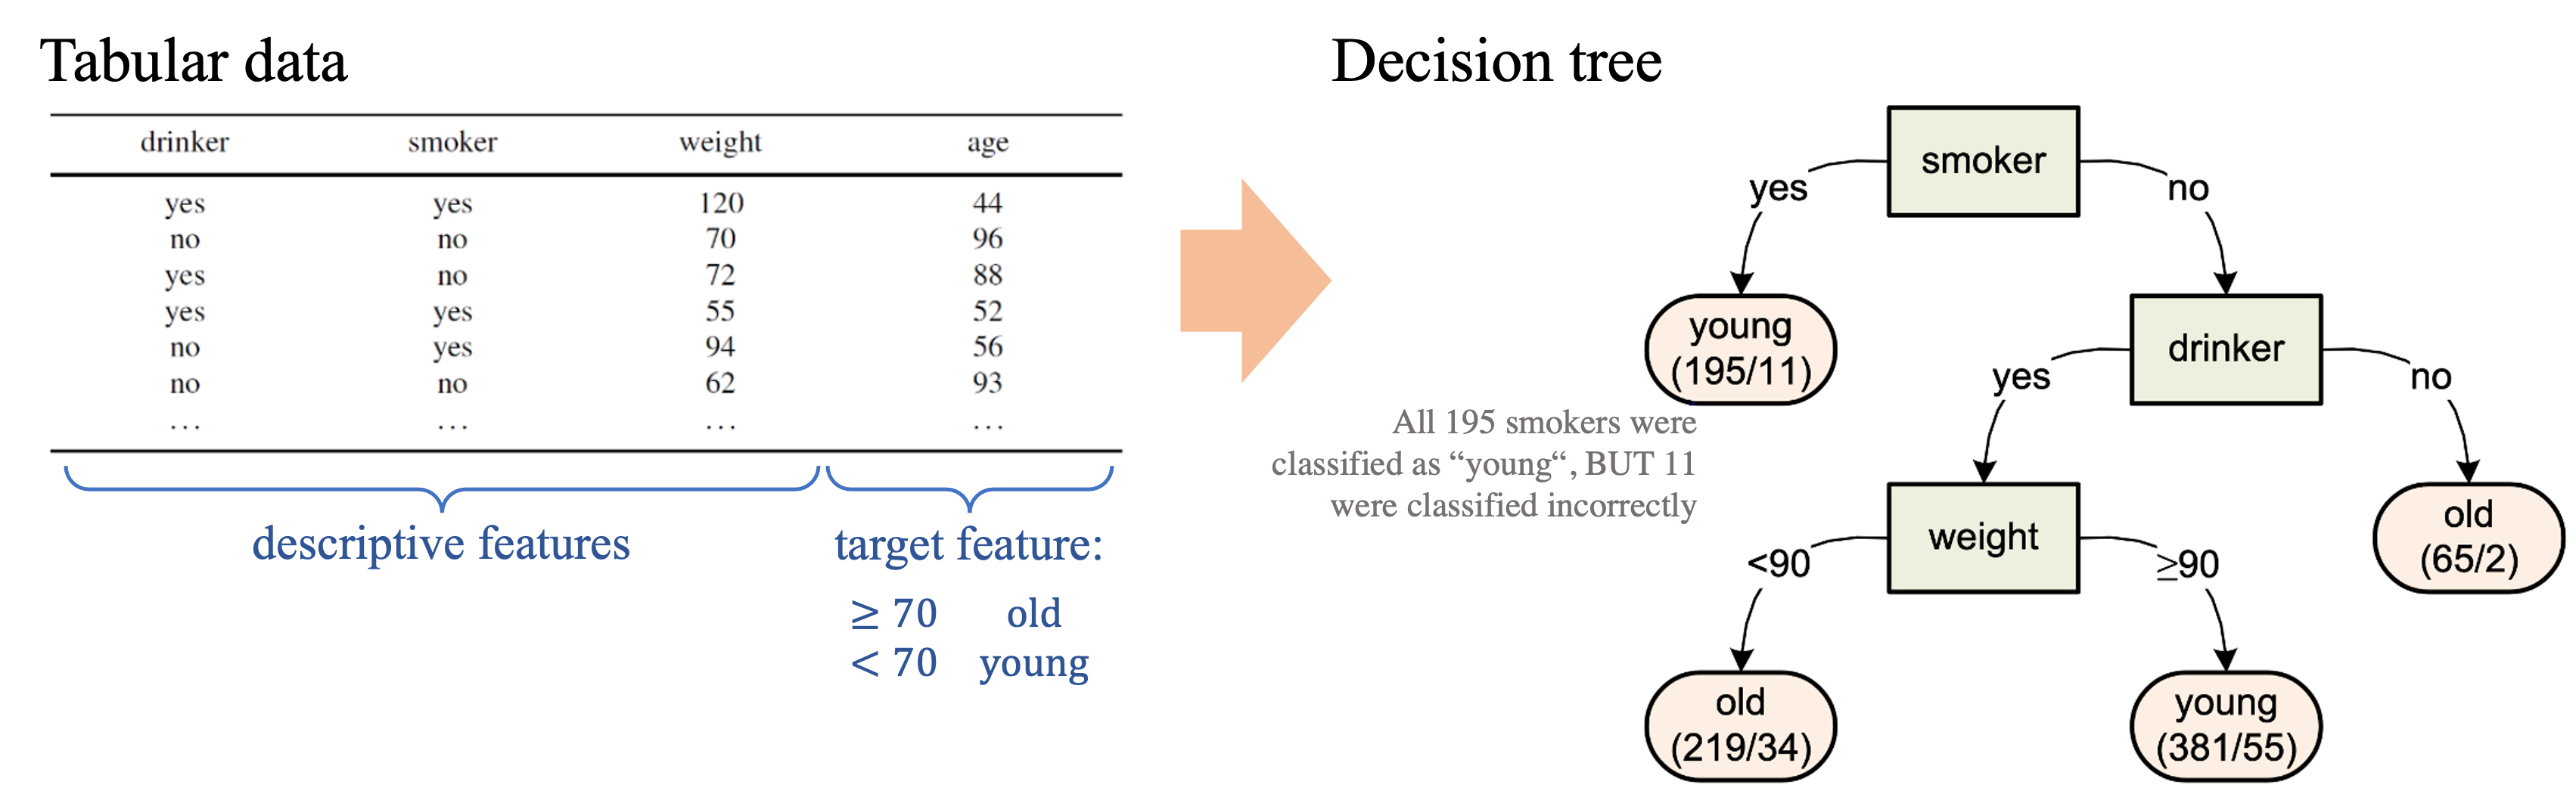
\includegraphics[width=\textwidth]{assets/trees/basics/tab_to_tree.png}
  \caption{Example for deriving a decision tree from tabular data (life expectancy)}
  \label{fig:3_smoke_tree_example}
\end{figure}

So summarized, a decision tree consists of three different types of nodes:\sidenote{Decision tree components}
\begin{itemize}
  \item A \textbf{root node} referring to all instances,
  \item \textbf{Interior nodes} partitioning the set of instances based on a descriptive feature, and
  \item \textbf{Leaf nodes} that have a label (the target feature value) that hopefully corresponds to a homogeneous group of instances with the same label.
\end{itemize}

How the partitioning influences the size and therefore efficiency of the decision tree can be seen in the example in \ref{fig:3_partitioning_example}. Both the good and bad partitioning options classify the observed instances correctly, but one is more simple and seems better. While investigating the example, keep the following keywords in mind:\sidenote{Partitioning keywords}
\begin{itemize}
  \item Avoid overfitting
  \item Apply Occam's razor \textcolor{gray}{\footnotesize (problem-solving principle recommending searching for explanation constructed with the smallest possible set of elements = simplest solution is best one)}
  \item Prefer shallow trees
\end{itemize}

\begin{figure}[h]
  \centering
  \begin{subfigure}{0.5\textwidth}
    \centering
    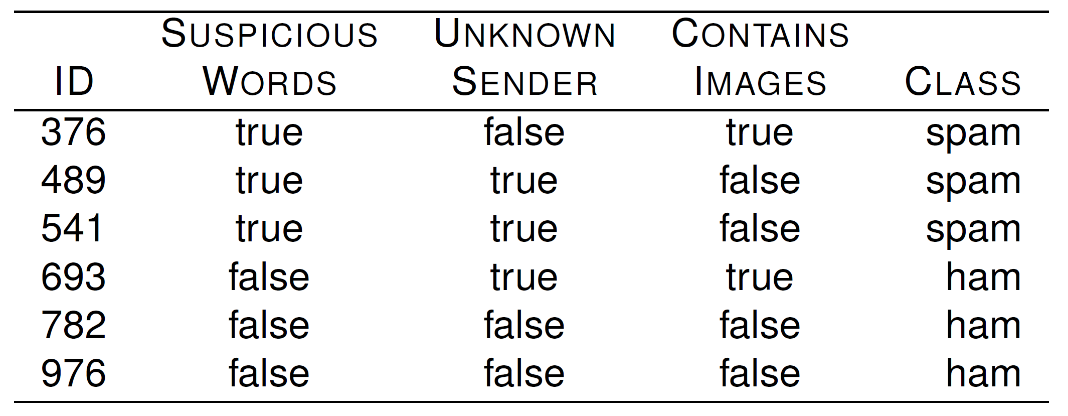
\includegraphics[width=0.9\textwidth]{assets/trees/basics/part_example_data.png}
    \subcaption{Tabular data}
  \end{subfigure}

  \hspace*{0.5cm}
  \begin{subfigure}{0.45\textwidth}
    \centering
    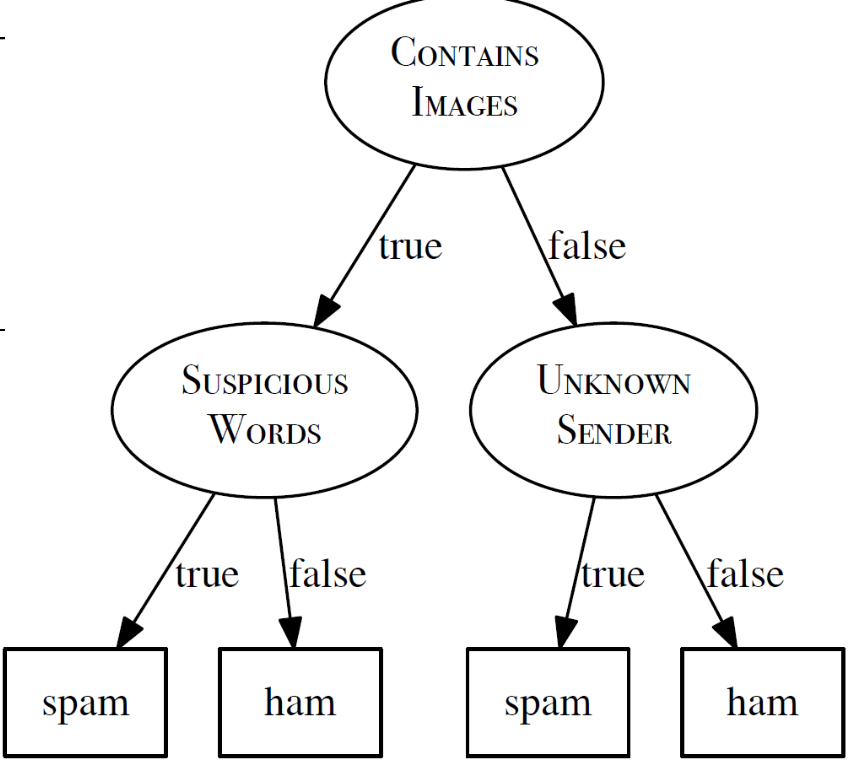
\includegraphics[width=0.9\textwidth]{assets/trees/basics/part_example_bad.png}
    \subcaption{"Bad" partitioning}
  \end{subfigure}
  \vspace*{10mm}
  \begin{subfigure}{0.45\textwidth}
    \centering
    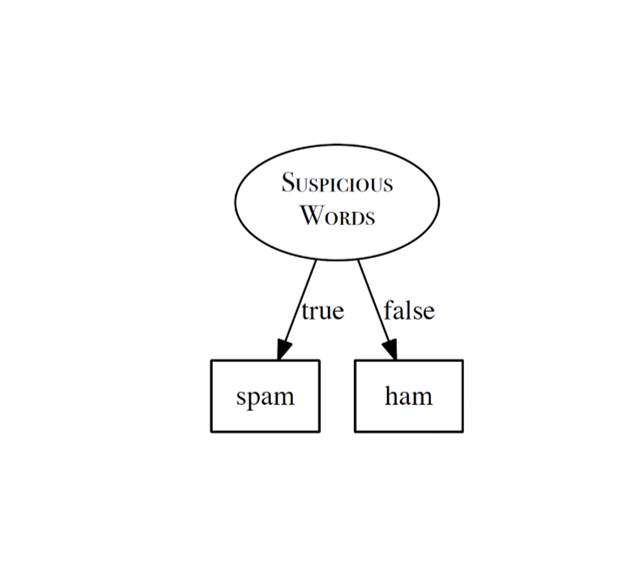
\includegraphics[width=0.9\textwidth]{assets/trees/basics/part_example_good.png}
    \subcaption{"Good" partitioning {\small(fewer decisions)}}
  \end{subfigure}
  \caption{Example for different partitioning results on the same problem (both correct)}
  \label{fig:3_partitioning_example}
\end{figure}
